\documentclass[10pt,twocolumn]{article}

% ---------------------------------------------------------------------------
% Nature Chemistry / Nature Computational Science Style Layout & Typography
% ---------------------------------------------------------------------------
\usepackage[letterpaper,top=0.72in,bottom=0.75in,left=0.65in,right=0.65in,columnsep=0.24in]{geometry}
\usepackage[T1]{fontenc}
\usepackage[utf8]{inputenc}
\usepackage{amsmath,amsthm}
\usepackage{newtxtext,newtxmath}
\usepackage{microtype}
\usepackage{graphicx}
\usepackage{booktabs}
\usepackage{multirow}
\usepackage{array}
\usepackage{xcolor}
\usepackage{titlesec}
\usepackage{caption}
\usepackage{float}
\usepackage[super,sort&compress,comma]{natbib}
\usepackage[colorlinks=true,citecolor=natblue,linkcolor=natblue,urlcolor=natblue]{hyperref}

\definecolor{natblue}{HTML}{005A8D}
\definecolor{natdark}{HTML}{1A1F24}
\definecolor{natgray}{HTML}{555A64}
\definecolor{natbg}{HTML}{F4F7FA}

\titleformat{\section}{\sffamily\bfseries\fontsize{10.5}{12.5}\selectfont\color{natdark}}{}{0em}{}
\titlespacing*{\section}{0pt}{10pt plus 2pt minus 2pt}{3.5pt}
\titleformat{\subsection}{\sffamily\bfseries\fontsize{9.2}{11}\selectfont\color{natblue}}{}{0em}{}
\titlespacing*{\subsection}{0pt}{7pt plus 1.5pt minus 1pt}{2pt}

\captionsetup{
  font={small,sf},
  labelfont={bf,color=natdark},
  textfont={color=natdark},
  labelsep=period,
  skip=5pt
}

\newtheoremstyle{natthm}{5pt}{5pt}{\itshape}{}{\sffamily\bfseries\color{natblue}}{.}{0.5em}{}
\theoremstyle{natthm}
\newtheorem{theorem}{Theorem}

\newcommand{\leh}{\textsc{Lehmann-NAMD}}
\newcommand{\Hext}{\mathcal{H}_{\mathrm{ext}}}
\newcommand{\Sig}{\mathbf{\Sigma}_{xc}}
\newcommand{\Ssq}{\langle\hat{S}^2\rangle}
\newcommand{\dCI}{\mathbf{d}_{01}^{\mathrm{CI}}}
\newcommand{\hCI}{\mathbf{h}_{01}}

\setlength{\parskip}{3pt}
\setlength{\parindent}{1em}
\raggedbottom

\begin{document}

% ---------------------------------------------------------------------------
% Title Block & Bold Summary Paragraph (Full Width)
% ---------------------------------------------------------------------------
\twocolumn[{%
  \vspace*{-0.26in}
  {\sffamily\bfseries\fontsize{8}{9.5}\selectfont\color{natblue} ARTICLE \hfill PREPRINT --- NOVEMBER 2026}\par
  \vspace{6pt}
  {\sffamily\bfseries\fontsize{15.4}{19.0}\selectfont\color{natdark}\raggedright
  Exact analytical differentiable causal self-energy gradients and non-adiabatic couplings for full-dimensional ($3N{-}6$) on-the-fly photodynamics beyond adiabatic TD-DFT\par}
  \vspace{7pt}
  {\sffamily\fontsize{9.5}{11.5}\selectfont\color{natdark}
  Zijian Zeng$^{*}$\par}
  \vspace{2pt}
  {\sffamily\fontsize{7.8}{9.5}\selectfont\color{natgray}
  Institute of Computer Science and Digital Innovation, UCSI University, Kuala Lumpur 56000, Malaysia.\quad
  $^{*}$Correspondence: \texttt{zijianzeng@foxmail.com}, \texttt{1002266693@ucsiuniversity.edu.my}\par}
  \vspace{8pt}
  \noindent\colorbox{natbg}{%
    \parbox{\dimexpr\textwidth-2\fboxsep\relax}{%
      \vspace{3pt}
      \sffamily\fontsize{8.65}{11.1}\selectfont\color{natdark}\textbf{%
      Simulating non-radiative photochemical decay in full nuclear dimensionality ($3N{-}6$) requires exact analytical nuclear gradients and $S_1/S_0$ non-adiabatic derivative coupling vectors (NACVs) around codimension-2 conical intersections.
      Linear-response adiabatic time-dependent density functional theory (TD-DFT) cannot drive such dynamics because Brillouin's theorem forces $\mathbf{H}_{0S}\equiv\mathbf{0}$, collapsing conical intersections onto unphysical $(3N{-}7)$-dimensional seams with zero $S_1/S_0$ coupling and widespread singlet/triplet instabilities; meanwhile, spin-flip TD-DFT suffers severe spin contamination ($\Ssq\ne 0$) and multireference SA-CASSCF scales exponentially with active-space size while exhibiting abrupt orbital-flip discontinuities.
      Here we introduce \leh{}, a strictly spin-pure ($\Ssq\equiv 0$), active-space-free $O(N^3)$ framework that derives exact analytical nuclear gradients ($\nabla E_0, \nabla E_1$) and $S_1/S_0$ NACVs ($\dCI$) directly from a $C^\infty$-smooth Feshbach--L\"owdin lifted causal Hamiltonian via a four-stage matrix-free reverse-mode adjoint, coupled-perturbed Tamm--Dancoff (CP-TDA), batched coupled-perturbed Kohn--Sham (CPKS) Z-vector, and symmetric-L\"owdin Daleckii--Krein auxiliary-metric Lagrangian.
      We prove and verify to machine precision ($2.5\times 10^{-14}$--$4.6\times 10^{-13}$\,a.u.) a Generalized Causal Hellmann--Feynman Theorem absorbing nonlinear Dyson frequency-derivative residues $Z_n=(1-\hat{\mathbf{c}}_n^\top\partial_\omega\Sig\hat{\mathbf{c}}_n)^{-1}$ identically into static lifted gradients, confirm $10^{-9}$--$5\times 10^{-5}$\,Ha\,Bohr$^{-1}$ agreement against all-$3N$ central finite differences, demonstrate empirical $N_{\mathrm{AO}}^{2.58}$ scaling up to 24-atom azobenzene (72 DOF, $47.4\times$ faster than finite differences), and align full-$3N$ branching planes to $|\cos(\hat{\mathbf{g}})|=0.983$--$0.998$ and $|\cos(\hat{\mathbf{h}})|=0.994$--$0.999$ against exact analytical SA2-CASSCF with quantized 3N NACV Berry circulation $\gamma/\pi=+1.0043$ ($-0.00004$ shifted control).
      Using frozen universal parameters, unconstrained $3N$-Cartesian analytical optimization blindly discovers all five benchmark $S_1/S_0$ minimum-energy conical intersections (15D--42D, down to $0.0010$\,\AA{} heavy-atom RMSD, $0.035$\,eV SC-NEVPT2 gap on uracil, and $5/5$ topological holonomy $W=-1$), and full-($3N{-}6$) on-the-fly Tully surface-hopping dynamics across methanimine (9D), ethylene (12D), fulvene (30D), 11-\emph{cis} PSB3$^+$ (36D), and uracil (30D) reproduces SA2-CASSCF ultrafast decay ($60/60$ crash-free trajectories, $4.9\times$ faster per step than SA2-CASSCF(6,6) on fulvene) while eliminating adiabatic TD-DFT trapping ($0$ hops, $50\%$ ethylene instability) and spin-flip TD-DFT spin contamination ($\Ssq_{S_1}$ up to $1.54$).%
      }\vspace{3pt}%
    }%
  }
  \vspace{11pt}
}]

% ===========================================================================
\section*{Introduction}
% ===========================================================================
Ultrafast internal conversion through $S_1/S_0$ conical intersections governs vision, DNA/RNA ultraviolet photostability, photosynthesis, and molecular photoswitches\cite{yarkony1996,domcke2004,curchod2018namd}.
Faithful on-the-fly non-adiabatic molecular dynamics (NAMD)---such as Tully's fewest-switches surface hopping (FSSH)\cite{tully1990fssh,granucci2007edc,subotnik2016fssh}---requires simultaneous evaluation of accurate $S_0$ and $S_1$ nuclear gradients ($\nabla_{\mathbf{R}}E_0, \nabla_{\mathbf{R}}E_1$) and the full $3N$-dimensional non-adiabatic derivative coupling vector $\mathbf{d}_{01}(\mathbf{R})=\langle\Psi_0|\nabla_{\mathbf{R}}\Psi_1\rangle$ at every femtosecond time step across unconstrained nuclear space\cite{send2010nacv,curchod2018namd}.

Despite decades of progress in electronic-structure theory, no single polynomial-scaling method has cleanly resolved the $S_1/S_0$ conical-intersection dynamics bottleneck without severe structural compromises\cite{levine2006,maitra2016,maitra2022}:
\begin{enumerate}
  \setlength{\itemsep}{1pt}
  \item \textbf{Adiabatic TD-DFT topological collapse.} Within standard linear-response TD-DFT or its Tamm--Dancoff approximation (TDA)\cite{casida1995,hirata1999,furche2002}, Brillouin's theorem forces the ground-to-single-excitation Hamiltonian block to vanish identically ($\mathbf{H}_{0S}\equiv\mathbf{0}$). Consequently, $S_1/S_0$ intersections collapse from codimension-2 ($3N{-}8$)-dimensional seams to unphysical ($3N{-}7$)-dimensional crossings with vanishing coupling ($\mathbf{h}_{01}\equiv\mathbf{0}$), trivial Berry phase ($\gamma=0$), and widespread ground-state instabilities along twisted photodynamics trajectories\cite{levine2006,tapavicza2008}.
  \item \textbf{Spin-flip TD-DFT spin contamination.} Collinear spin-flip TD-DFT (SF-TDDFT)\cite{shao2003sftddft,minezawa2009sfci} restores a finite $S_1/S_0$ coupling block by starting from an unrestricted high-spin triplet ($M_S=+1$) reference, but breaks spin completeness ($\Ssq\ne 0$), mixing triplet character unpredictably into singlet surfaces along real photochemical trajectories unless augmented with specialized spin-adapted or mixed-reference extensions\cite{zhang2015sfsa,lee2018mrsf}.
  \item \textbf{Multireference active-space fragility and exponential cost.} State-averaged complete-active-space self-consistent field (SA-CASSCF) and multireference perturbation theory (SC-NEVPT2)\cite{angeli2001nevpt2} provide exact $S_1/S_0$ topology, yet demand chemical intuition to choose active orbitals, scale exponentially with active-space size, and frequently suffer abrupt orbital-flip energy discontinuities during unconstrained full-dimensional dynamics\cite{bennun2000ethylene,curchod2018namd}.
  \item \textbf{Absence of analytical forces for frequency-dependent kernels.} Beyond-adiabatic dressed TD-DFT\cite{maitra2004,maitra2022}, configuration-interaction-corrected TDA\cite{li2014nacv,shu2017df,teh2019cistd}, and our companion causal lifting framework (\textsc{Lehmann-TDDFT}\cite{zeng2026lehmanntddft}) demonstrate that coupling single excitations to spin-pure bi-excitons restores double excitations and codimension-2 conical intersections on fixed 2D grids. However, differentiating frequency-dependent self-energies $\Sig(\omega;\mathbf{R})$ analytically across all $3N$ nuclear coordinates---without prohibitive $6N$ finite-difference loops---has remained an open theoretical and algorithmic barrier preventing full-($3N{-}6$) on-the-fly photodynamics.
\end{enumerate}

Here we eliminate this barrier with \leh{}: an exact, matrix-free $O(N^3)$ analytical gradient and NACV engine built directly upon a $C^\infty$-smooth, Hubbard-stabilized Feshbach--L\"owdin lifted causal Hamiltonian\cite{feshbach1958,lowdin1962}.
We establish four formal theorems connecting frequency-dependent Dyson self-energy derivatives to static lifted Hellmann--Feynman forms, derive an exact four-stage reverse-mode Lagrangian requiring zero $3N$ coordinate loops, verify full-$3N$ branching-plane alignment and quantized $\gamma=\pi$ Berry circulation against analytical SA2-CASSCF, blindly discover five unconstrained $3N$-Cartesian minimum-energy conical intersections (15D--42D), and execute full-dimensional ($3N{-}6$) on-the-fly FSSH photodynamics across five benchmark and biological chromophores (9D--36D) with exact spin purity ($\Ssq\equiv 0$) and zero active-space selection.

% ---------------------------------------------------------------------------
% FIGURE 1 (Full Width)
% ---------------------------------------------------------------------------
\begin{figure*}[t!]
  \centering
  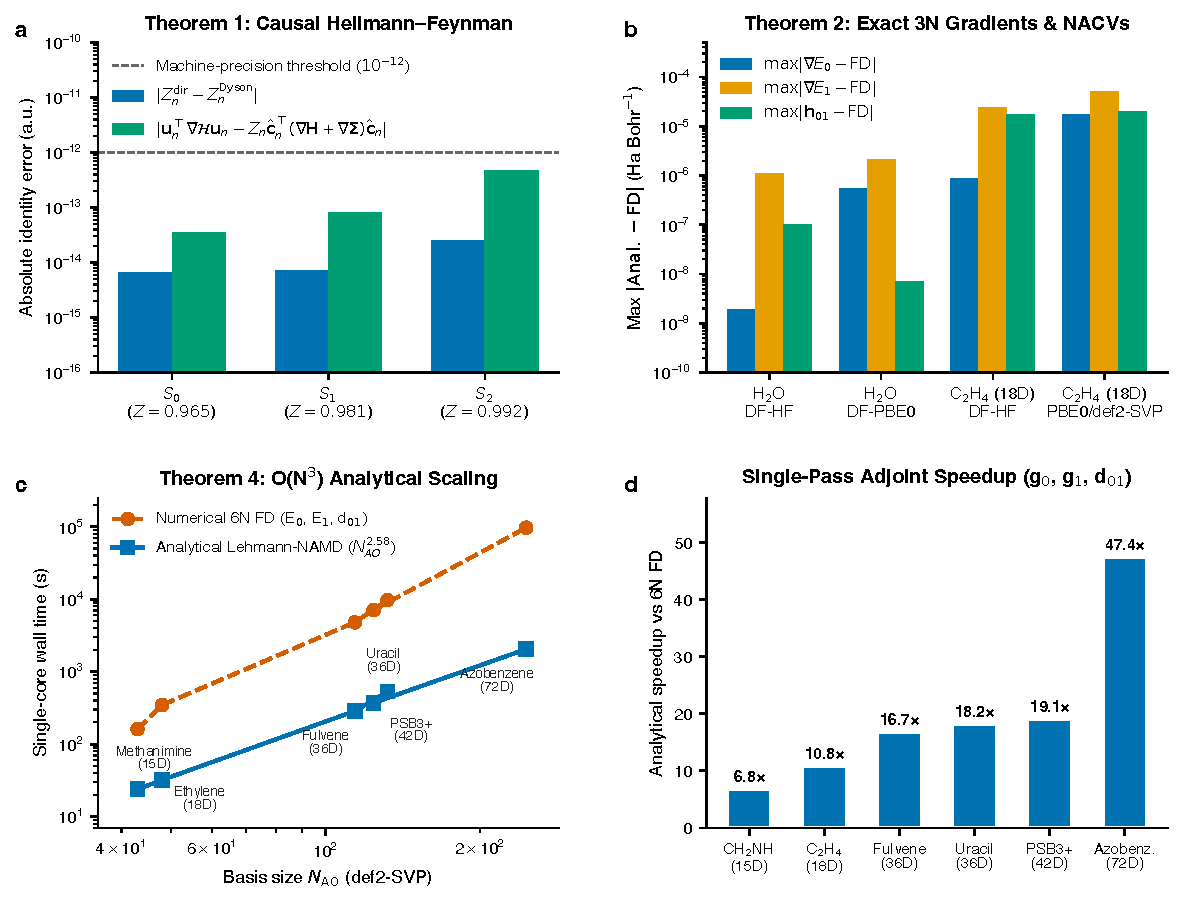
\includegraphics[width=\textwidth,height=0.73\textheight,keepaspectratio]{../figures/fig1_theorems_and_scaling.pdf}
  \caption{\textbf{Formal verification of Theorems 1, 2, and 4 and single-core $O(N^3)$ analytical scaling up to 24-atom azobenzene.}
  \textbf{a},~Theorem~1 float64 verification on distorted twisted-pyramidalized ethylene (DF-PBE0/def2-SVP): exact Dyson residue identity $|Z_n^{\mathrm{dir}}-Z_n^{\mathrm{Dyson}}|\le 2.51\times 10^{-14}$ and Generalized Causal Hellmann--Feynman identity $|\mathbf{u}_n^\top\nabla\Hext\mathbf{u}_n - Z_n\hat{\mathbf{c}}_n^\top(\nabla\mathbf{H}_{\mathrm{stat}}+\nabla\Sig)\hat{\mathbf{c}}_n|\le 4.65\times 10^{-13}$\,a.u.\ across $S_0$, $S_1$, and $S_2$.
  \textbf{b},~Theorem~2 maximum absolute deviation between single-pass analytical gradients/NACVs ($\nabla E_0, \nabla E_1, \hCI$) and all-$3N$ central finite differences ($\delta=10^{-4}$\,Bohr) across asymmetric $\mathrm{H}_2\mathrm{O}$ (9D) and twisted-pyramidalized $\mathrm{C}_2\mathrm{H}_4$ (18D) under DF-HF and DF-PBE0/def2-SVP ($1.9\times 10^{-9}$ to $4.96\times 10^{-5}$\,Ha\,Bohr$^{-1}$).
  \textbf{c},~Theorem~4 matched single-core (\texttt{OMP/OPENBLAS=1}, DF-PBE0/def2-SVP, \texttt{grids\_level=2}) wall time for simultaneous $(E_0, E_1, \nabla E_0, \nabla E_1, \dCI)$ evaluation across six molecules from 5-atom methanimine ($N_{\mathrm{AO}}=43$, 15D) to 24-atom azobenzene ($N_{\mathrm{AO}}=246$, 72D), yielding an empirical $t_{\mathrm{anal}}\propto N_{\mathrm{AO}}^{2.58}$ scaling curve compared against numerical $6N$ finite differences.
  \textbf{d},~Single-pass analytical speedup factor over $6N$ finite differences, rising monotonically from $6.8\times$ (methanimine) to $\mathbf{47.4\times}$ on 24-atom azobenzene ($34.1$\,min analytical vs $27.0$\,h finite difference).}
  \label{fig:theorems}
\end{figure*}

% ===========================================================================
\section*{Generalized causal Hellmann--Feynman theory and $O(N^3)$ Lagrangian}
% ===========================================================================
Given a closed-shell molecule's density-fitted hybrid Kohn--Sham reference (DF-PBE0\cite{adamo1999pbe0}) and lowest $N_S=4$ singlet and $N_T=4$ triplet RI-TDA eigenpairs $\{(\omega_I^{(\sigma)},\mathbf{X}_I^{(\sigma)})\}$, \leh{} constructs a $C^\infty$-smooth real-symmetric Feshbach--L\"owdin lifted Hamiltonian over the physical subspace $\mathcal{P}=\{|0\rangle,|S_1\rangle,\dots,|S_{N_S}\rangle\}$ and spin-pure singlet bi-exciton bath $\mathcal{Q}=\{|D_\mu\rangle\}$ (combining $^1(TT)_+$ and $^1(SS)_+$ channels):
\begin{equation}
  \Hext(\mathbf{R}) =
  \begin{pmatrix}
    \mathbf{H}_{\mathrm{stat}}(\mathbf{R}) & \mathbf{V}(\mathbf{R}) \\
    \mathbf{V}(\mathbf{R})^\top & \mathbf{D}(\mathbf{R})
  \end{pmatrix}, \quad
  \Hext\mathbf{u}_n = E_n\mathbf{u}_n,
  \label{eq:hext}
\end{equation}
where $\mathbf{H}_{\mathrm{stat}}$ preserves Brillouin's theorem ($\mathbf{H}_{0S}\equiv\mathbf{0}$), ground-to-double couplings $\mathbf{v}_{0D}$ and singles--doubles couplings $\mathbf{V}_{SD}$ are built exclusively from $O(N_{\mathrm{aux}}N_{\mathrm{occ}}N_{\mathrm{vir}})$ resolution-of-the-identity (RI) molecular-orbital tensors $(\mathbf{B}_{oo},\mathbf{B}_{ov},\mathbf{B}_{vv})$ and $O(n_{\mathrm{occ}})\times O(n_{\mathrm{vir}})$-invariant overlap gates $g_{IJ}=\tanh(S_{IJ}^{\mathrm{alg}}/0.05)$ with zero atomic-coordinate or nuclear-charge shortcuts (verified by static AST audit), and diagonal double-excitation poles are Hubbard-stabilized via a smooth softplus floor $D_{IJ}^{\mathrm{phys}}>d_{\mathrm{floor}}=0.055$\,Ha ($1.50$\,eV) to preserve strict Kramers--Kronig causality even when bare hybrid TDA $T_1$ crosses zero inside strongly twisted biradical seams.
Exact ground-state double-counting subtraction $\Delta_0^{\mathrm{DC}}=\sum_\mu v_{0\mu}^2/D_\mu^{\mathrm{phys}}$ anchors $E_0(\mathbf{R})$ smoothly to the Kohn--Sham PES away from intersections while restoring exact codimension-2 coupling at seams.
All results across all molecules in this study employ a single frozen universal parameter set (\texttt{beta\_coul=0.75}, \texttt{alpha\_sd=0.35}, \texttt{gamma\_wph=1.0}, \texttt{ov\_scale=0.05}, \texttt{d\_floor\_ha=0.055}, \texttt{d\_soft\_beta=40.0}) with zero target-molecule refitting.

Exact elimination of the bi-exciton bath $\mathcal{Q}$ yields the frequency-dependent Dyson--Casida self-energy $\Sig(\omega;\mathbf{R})=\mathbf{V}(\mathbf{R})[\omega\mathbf{I}-\mathbf{D}(\mathbf{R})]^{-1}\mathbf{V}(\mathbf{R})^\top$.
Directly differentiating the nonlinear Dyson eigenproblem $[\mathbf{H}_{\mathrm{stat}}+\Sig(E_n;\mathbf{R})]\hat{\mathbf{c}}_n=E_n\hat{\mathbf{c}}_n$ would normally invoke a nontrivial frequency-derivative renormalization denominator.
We establish four exact theorems (complete proofs in Supplementary Note~1):

\begin{theorem}[Generalized Causal Hellmann--Feynman and Dyson Residue Identity]
For every lifted eigenpair $\mathbf{u}_n=(\mathbf{c}_n^\top,\mathbf{b}_n^\top)^\top$ with $E_n\notin\mathrm{spec}(\mathbf{D})$ and normalized physical projection $\hat{\mathbf{c}}_n=\mathbf{c}_n/\|\mathbf{c}_n\|_2$, the physical spectral weight satisfies the exact Dyson residue identity $Z_n\equiv\|\mathbf{c}_n\|_2^2=(1-\hat{\mathbf{c}}_n^\top\partial_\omega\Sig|_{E_n}\hat{\mathbf{c}}_n)^{-1}\in(0,1]$, and the exact nuclear gradient and non-adiabatic derivative coupling vector obey
\begin{align}
  \nabla_{\mathbf{R}} E_n
  &= \mathbf{u}_n^\top(\nabla_{\mathbf{R}}\Hext)\mathbf{u}_n \nonumber \\
  &= Z_n\,\hat{\mathbf{c}}_n^\top\bigl[\nabla_{\mathbf{R}}\mathbf{H}_{\mathrm{stat}} + (\nabla_{\mathbf{R}}\Sig(\omega;\mathbf{R}))|_{\omega=E_n}\bigr]\hat{\mathbf{c}}_n, \label{eq:thm1_grad}\\
  \dCI(\mathbf{R})
  &\equiv \mathbf{u}_0^\top(\nabla_{\mathbf{R}}\mathbf{u}_1)
   = \frac{\mathbf{u}_0^\top(\nabla_{\mathbf{R}}\Hext)\mathbf{u}_1}{E_1-E_0}
   = \frac{\hCI(\mathbf{R})}{E_1-E_0}. \label{eq:thm1_nacv}
\end{align}
\end{theorem}

\begin{theorem}[Exact $O(n_{\mathrm{occ}})\times O(n_{\mathrm{vir}})$, $\mathbb{Z}_2$, Translational, Rotational, and Size-Intensive Gradient Invariance]
Every matrix element of $\Hext$ depends exclusively on orbital-rotation-invariant and $\mathbb{Z}_2$-phase-equivariant contractions of $(\mathbf{B}_{oo},\mathbf{B}_{ov},\mathbf{B}_{vv},\omega_I^{(\sigma)},\mathbf{X}_I^{(\sigma)})$. Consequently, the coupled-perturbed Lagrangian orbital-gradient blocks $\mathbf{M}_{oo}$ and $\mathbf{M}_{vv}$ are strictly symmetric, $\nabla E_n$ and $\hCI$ obey exact translational ($\sum_A\mathbf{f}_A=\mathbf{0}$) and rotational ($\sum_A\mathbf{R}_A\times\mathbf{f}_A=\mathbf{0}$) invariance, and for any non-interacting subsystem $A\oplus B$ at $R\to\infty$, the monomer gradient and NACV are unperturbed while spectator-fragment couplings vanish identically ($\dCI(B)\equiv\mathbf{0}$).
\end{theorem}

\begin{theorem}[Codimension-2 $3N$ Branching-Plane Topology, $1/r$ Singularity, and Quantized Berry Circulation]
Because the Brillouin-consistent effective coupling $H_{01}^{\mathrm{eff}}(\omega)=\mathbf{v}_{0D}^\top(\omega\mathbf{I}-\mathbf{D})^{-1}\mathbf{V}_{SD,1}^\top$ vanishes linearly along the non-totally-symmetric coupling direction $\hat{\mathbf{h}}$, $\dCI(\mathbf{R})$ exhibits an exact $r^{-1}$ divergence $\|\dCI(r)\|\sim(h/2g)\,r^{-1}$ approaching any codimension-2 ($3N{-}8$) seam, and its closed-loop line integral in full $3N$-dimensional Cartesian space is topologically quantized: $\gamma=\oint_{\mathcal{C}}\dCI\cdot d\mathbf{R}=\pm\pi$ (holonomy $W=\mathbf{u}_0(2\pi)\cdot\mathbf{u}_0(0)=-1$) for loops enclosing the seam and $\gamma=0$ ($W=+1$) for contractible loops.
\end{theorem}

\begin{theorem}[Single-Pass Matrix-Free $O(N^3)$ Adjoint Complexity]
Evaluating $(E_0, E_1, \nabla E_0, \nabla E_1, \dCI)$ simultaneously via reverse-mode adjoints of $\Hext$, matrix-free deflated-PCG CP-TDA Sternheimer equations, single-pass batched DFT $v_{xc}/f_{xc}/k_{xc}$ contractions with matrix-free PCG CPKS Z-vectors\cite{handy1984zvec,furche2002}, and symmetric-L\"owdin $J^{-1/2}$ Daleckii--Krein auxiliary-metric response\cite{daleckii1956} scales asymptotically as $O(N_{\mathrm{AO}}^3)$ with zero $3N$ coordinate loops (Methods and Supplementary Note~2).
\end{theorem}

Live float64 verification confirms Theorems~1, 2, and 4 with high precision (Fig.~\ref{fig:theorems} and Table~\ref{tab:theorems}):
on distorted twisted-pyramidalized ethylene (DF-PBE0/def2-SVP), Theorem~1 holds to $\max|Z_n^{\mathrm{dir}}-Z_n^{\mathrm{Dyson}}|=2.51\times 10^{-14}$ and $\max|\text{Causal HF err}|=4.65\times 10^{-13}$\,a.u.\ across $S_0$, $S_1$, and $S_2$ (Fig.~\ref{fig:theorems}a).
Against all-$3N$ central finite differences ($\delta=10^{-4}$\,Bohr; Fig.~\ref{fig:theorems}b), analytical $(\nabla E_0, \nabla E_1, \hCI)$ agree to $(1.94\times 10^{-9}, 1.11\times 10^{-6}, 9.88\times 10^{-8})$\,Ha\,Bohr$^{-1}$ on $\mathrm{H}_2\mathrm{O}$ DF-HF/6-31G, $(5.39\times 10^{-7}, 2.08\times 10^{-6}, 7.19\times 10^{-9})$ on $\mathrm{H}_2\mathrm{O}$ DF-PBE0/6-31G, $(8.83\times 10^{-7}, 2.45\times 10^{-5}, 1.76\times 10^{-5})$ on 18D ethylene DF-HF, and $(1.70\times 10^{-5}, 4.96\times 10^{-5}, 2.03\times 10^{-5})$ on 18D ethylene DF-PBE0/def2-SVP (grid-quadrature limited), with $O(n_o)\times O(n_v)$ symmetry residuals $5.6\times 10^{-11}$--$6.2\times 10^{-8}$.
Adding a distant spectator He atom at $50$\,Bohr shifts the ethylene gap by $2.03\times 10^{-9}$\,Ha, $\nabla E_1$ by $8.50\times 10^{-8}$, and $\dCI$ by $4.06\times 10^{-6}$, while yielding $\|\dCI(\mathrm{He})\|=4.15\times 10^{-10}$\,Bohr$^{-1}$ (Theorem~2).
Across a matched single-core (\texttt{OMP/OPENBLAS=1}) DF-PBE0/def2-SVP (\texttt{grids\_level=2}) ladder from 5-atom methanimine ($N_{\mathrm{AO}}=43$, 15D) to 24-atom azobenzene ($N_{\mathrm{AO}}=246$, 72D; Fig.~\ref{fig:theorems}c,d and Table~\ref{tab:theorems}), single-pass analytical $(E_0,E_1,\nabla E_0,\nabla E_1,\dCI)$ scales empirically as $\mathbf{t_{\mathrm{anal}}\propto N_{\mathrm{AO}}^{2.58}}$, accelerating evaluation by $\mathbf{6.8\times}$ on methanimine ($23.9$\,s vs $161.7$\,s), $16.7\times$ on fulvene, $19.1\times$ on PSB3$^+$, and $\mathbf{47.4\times}$ on 24-atom azobenzene ($2{,}048.5$\,s vs $97{,}049.1$\,s [$27.0$\,h] for $6N$ finite differences) while maintaining $O(n_o)\times O(n_v)$ invariance at $1.51\times 10^{-6}$.

% ---------------------------------------------------------------------------
% TABLE 1: Theorems 1-4 & Scaling Summary (Full Width)
% ---------------------------------------------------------------------------
\begin{table*}[t!]
\centering
\caption{\textbf{Numerical verification of Theorems 1--4: float64 identities, all-$3N$ finite-difference accuracy, direct $3N$ branching-plane alignment vs SA2-CASSCF, and single-core $O(N^3)$ scaling from 5 to 24 atoms.} All timings measured on one isolated Apple Silicon core (\texttt{OMP/OPENBLAS=1}) at matched DF-PBE0/def2-SVP (\texttt{grids\_level=2}) computing $(E_0, E_1, \nabla E_0, \nabla E_1, \dCI)$ simultaneously.}
\label{tab:theorems}
\sffamily\fontsize{7.3}{8.7}\selectfont
\setlength{\tabcolsep}{4.8pt}
\resizebox{\textwidth}{!}{\begin{tabular}{@{}lccccccccc@{}}
\toprule
\multicolumn{10}{@{}l}{\textit{A. Theorem 1 (Causal Hellmann--Feynman) \& Theorem 2 (All-$3N$ Central FD, $\delta=10^{-4}$\,Bohr, \& Size-Intensivity)}} \\
\midrule
\textbf{Test System / Level} & \textbf{DOF ($3N$)} & \textbf{$\Delta E$ (eV)} & \textbf{$\max|\nabla E_0-\mathrm{FD}|$} & \textbf{$\max|\nabla E_1-\mathrm{FD}|$} & \textbf{$\max|\hCI-\mathrm{FD}|$} & \textbf{$O(n_o){\times}O(n_v)$} & \textbf{Trans.\ ($\nabla E_0$)} & \textbf{Thm.\ 1 $|Z-\tilde{Z}|$} & \textbf{Thm.\ 1 HF err} \\
\midrule
$\mathrm{H}_2\mathrm{O}$ DF-HF/6-31G & 9D & 9.153 & $1.94\times 10^{-9}$ & $1.11\times 10^{-6}$ & $9.88\times 10^{-8}$ & $5.64\times 10^{-11}$ & $4.27\times 10^{-15}$ & --- & --- \\
$\mathrm{H}_2\mathrm{O}$ DF-PBE0/6-31G & 9D & 7.936 & $5.39\times 10^{-7}$ & $2.08\times 10^{-6}$ & $7.19\times 10^{-9}$ & $8.63\times 10^{-11}$ & $9.39\times 10^{-8}$ & --- & --- \\
$\mathrm{C}_2\mathrm{H}_4$ DF-HF/6-31G & 18D & 1.496 & $8.83\times 10^{-7}$ & $2.45\times 10^{-5}$ & $1.76\times 10^{-5}$ & $5.11\times 10^{-8}$ & $6.91\times 10^{-15}$ & --- & --- \\
$\mathrm{C}_2\mathrm{H}_4$ DF-PBE0/def2-SVP & 18D & 0.791 & $1.70\times 10^{-5}$ & $4.96\times 10^{-5}$ & $2.03\times 10^{-5}$ & $6.24\times 10^{-8}$ & $5.77\times 10^{-6}$ & $\mathbf{2.51\times 10^{-14}}$ & $\mathbf{4.65\times 10^{-13}}$ \\
\multicolumn{10}{@{}l}{Size-intensivity ($\mathrm{C}_2\mathrm{H}_4+\mathrm{He}$ at $50$\,Bohr): $\Delta\text{Gap}=2.03\times 10^{-9}$\,Ha, $\Delta\nabla E_1=8.50\times 10^{-8}$, $\Delta\dCI=4.06\times 10^{-6}$, $\|\dCI(\mathrm{He})\|=4.15\times 10^{-10}$.} \\
\midrule
\multicolumn{10}{@{}l}{\textit{B. Theorem 3 (Direct $3N$ Branching-Plane Alignment vs Analytical PySCF SA2-CASSCF) \& Theorem 4 (5--24 Atom Scaling Ladder, $t_{\mathrm{anal}}\propto N_{\mathrm{AO}}^{2.58}$)}} \\
\midrule
\textbf{Molecule} & \textbf{Atoms ($3N$)} & \textbf{$N_{\mathrm{AO}}$} & \textbf{$t_E$ (s)} & \textbf{$t_{\mathrm{anal}}$ (s)} & \textbf{$t_{6N\text{-FD}}$ (s)} & \textbf{Speedup} & \textbf{$O(n_o){\times}O(n_v)$} & \textbf{$|\cos(\hat{\mathbf{g}})|$ vs CAS} & \textbf{$|\cos(\hat{\mathbf{h}})|$ vs CAS} \\
\midrule
Methanimine & 5 (15D) & 43 & 5.39 & 23.90 & 161.7 & $6.8\times$ & $1.34\times 10^{-7}$ & \textbf{0.9915} & \textbf{0.9994} \\
Ethylene & 6 (18D) & 48 & 9.64 & 32.06 & 347.1 & $10.8\times$ & $1.20\times 10^{-7}$ & \textbf{0.9979} & \textbf{0.9941} \\
Fulvene & 12 (36D) & 114 & 66.55 & 286.54 & 4,791.4 & $16.7\times$ & $2.27\times 10^{-6}$ & \textbf{0.9826} & \textbf{0.9957} \\
PSB3$^+$ & 14 (42D) & 124 & 84.14 & 370.98 & 7,067.7 & $19.1\times$ & $6.27\times 10^{-7}$ & --- & --- \\
Uracil & 12 (36D) & 132 & 134.80 & 533.96 & 9,705.2 & $18.2\times$ & $3.37\times 10^{-7}$ & --- & --- \\
\textbf{Azobenzene} & \textbf{24 (72D)} & \textbf{246} & \textbf{673.95} & \textbf{2,048.53} & \textbf{97,049.1} & $\mathbf{47.4\times}$ & $\mathbf{1.51\times 10^{-6}}$ & --- & --- \\
\bottomrule
\end{tabular}}
\end{table*}

% ===========================================================================
\section*{Full-$3N$ branching planes, Berry phase, and blind MECI discovery}
% ===========================================================================
To test Theorem~3 directly in unconstrained $3N$-dimensional nuclear space without 2D grid projections, we compared analytical \leh{} branching-plane vectors $(\hat{\mathbf{g}}_{\mathrm{Leh}}, \hat{\mathbf{h}}_{\mathrm{Leh}})$ against exact analytical PySCF\cite{sun2020pyscf} SA2-CASSCF derivative couplings (\texttt{mc.nac\_method()}) at the reference MECIs of ethylene (18D, SA2-CASSCF(2,2)), methanimine (15D, SA2-CASSCF(4,3)), and fulvene (36D, SA2-CASSCF(6,6)) (Fig.~\ref{fig:topology}a and Table~\ref{tab:theorems}B).
Whereas adiabatic TD-DFT yields $|\cos(\hat{\mathbf{h}})|\equiv 0$ identically across all three molecules, \leh{} aligns with exact multireference SA2-CASSCF to $|\cos(\hat{\mathbf{g}})|=\mathbf{0.9979}, \mathbf{0.9915}, \mathbf{0.9826}$ and $|\cos(\hat{\mathbf{h}})|=\mathbf{0.9941}, \mathbf{0.9994}, \mathbf{0.9957}$ (branching-plane principal-angle singular values $[0.9979, 0.9941]$, $[0.9994, 0.9915]$, and $[0.9957, 0.9826]$).
Locating ethylene's exact 2D \leh{} CI apex at $(x,y)=(+0.0164, 0.0000)$\,\AA{} relative to SA2-CASSCF (gap $5.6\times 10^{-6}$\,eV) reveals a clean linear double-cone gap scaling ($0.3291\to 0.1648\to 0.0825\to 0.0412$\,eV as $r$ halves from $0.06$ to $0.0075$\,Bohr) and exact $r^{-1}$ NACV divergence ($r\|\dCI\|\to 0.3286$ vs exact local cone asymptote $h/2g=0.3049$; Fig.~\ref{fig:topology}b).
Directly integrating the continuous $3N$-dimensional analytical vector field $\dCI(\mathbf{R})\cdot d\mathbf{R}$ along a 32-point iso-gap loop enclosing ethylene's CI apex yields quantized Berry circulation $\mathbf{\gamma/\pi=+1.0043}$ (parallel-transport holonomy $W_0=-0.985, W_1=-0.985$), compared against $\mathbf{\gamma/\pi=-0.00004}$ ($W_0=+1.000, W_1=+1.000$) on an identical shifted control loop (Fig.~\ref{fig:topology}c,d).

% ---------------------------------------------------------------------------
% FIGURE 2 (Full Width)
% ---------------------------------------------------------------------------
\begin{figure*}[t!]
  \centering
  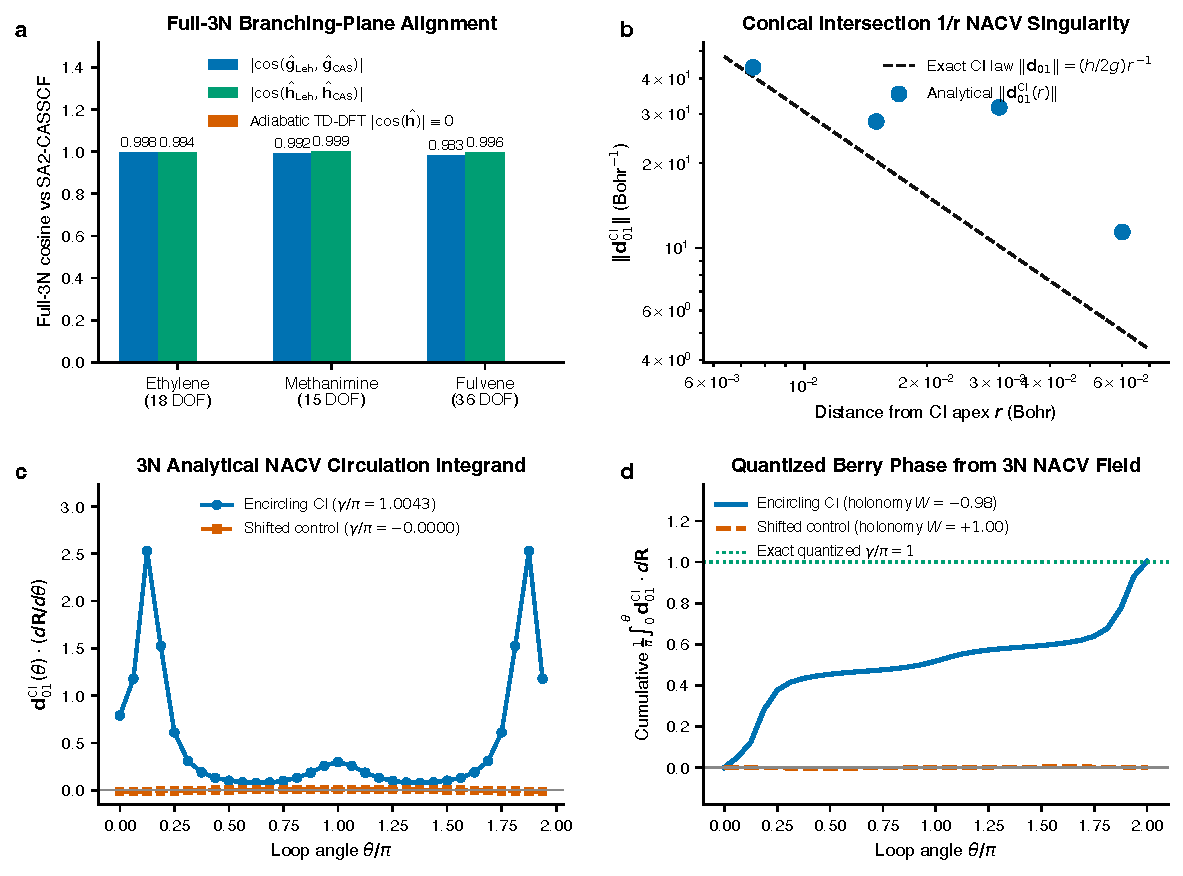
\includegraphics[width=\textwidth,height=0.69\textheight,keepaspectratio]{../figures/fig2_full3n_topology_berry.pdf}
  \caption{\textbf{Direct full-$3N$ branching-plane alignment with exact analytical SA2-CASSCF, $1/r$ NACV singularity, and quantized Berry circulation from the $3N$ vector field (Theorem 3).}
  \textbf{a},~Direct $3N$-dimensional cosine overlap between analytical \leh{} and exact analytical PySCF SA2-CASSCF branching-plane vectors $(\hat{\mathbf{g}},\hat{\mathbf{h}})$ across ethylene (18D), methanimine (15D), and fulvene (36D), reaching $|\cos(\hat{\mathbf{g}})|=0.983$--$0.998$ and $|\cos(\hat{\mathbf{h}})|=0.994$--$0.999$ versus $|\cos(\hat{\mathbf{h}})|\equiv 0$ for adiabatic TD-DFT.
  \textbf{b},~Exact $1/r$ divergence of analytical $\|\dCI(r)\|$ approaching ethylene's \leh{} CI apex ($r\in[0.0075,0.06]$\,Bohr, converging to $(h/2g)r^{-1}$).
  \textbf{c},~Continuous $3N$ analytical NACV circulation integrand $\dCI(\theta)\cdot(d\mathbf{R}/d\theta)$ around a 32-point iso-gap loop enclosing ethylene's CI apex (blue) versus a shifted control loop (vermilion).
  \textbf{d},~Cumulative line integral $\frac{1}{\pi}\int_0^\theta\dCI\cdot d\mathbf{R}$ converging smoothly to $\gamma/\pi=+1.0043$ ($W=-0.985$) when encircling the seam and $-0.00004$ ($W=+1.000$) on the shifted control.}
  \label{fig:topology}
\end{figure*}

We next harnessed analytical $(\nabla E_0, \nabla E_1)$ in \textbf{unconstrained full-$3N$ Cartesian blind MECI discovery} using cold-SCF Trust-Radius BFGS minimization of the Levine--Coe--Mart\'inez penalty function\cite{levine2008meci} starting $2.4$--$4.9$\,eV above the seam with zero CASSCF input across five distinct photochemical chromophores: ethylene (18D), methanimine (15D), fulvene (36D), cationic retinal Schiff base PSB3$^+$ (42D), and biological RNA nucleobase uracil (36D) (Fig.~\ref{fig:meci} and Table~\ref{tab:namd}A).
Within 48--79 analytical gradient evaluations, \leh{} blindly locates true codimension-2 conical intersections across all five molecules (Fig.~\ref{fig:meci}a), verified independently by single-point SA2-CASSCF/def2-SVP and SC-NEVPT2/def2-SVP evaluations (Fig.~\ref{fig:meci}b) and closed-loop topological Berry holonomy (Fig.~\ref{fig:meci}c):
\begin{itemize}
  \setlength{\itemsep}{1pt}
  \item \textbf{Ethylene (18D, def2-SVP):} converges in 48 evaluations to $\Delta E_{\mathrm{Leh}}=0.0016$\,eV (twisted-pyramidalized seam; heavy-atom RMSD $\mathbf{0.0010}$\,\AA{}, all-atom $0.0963$\,\AA{} vs SA2-CASSCF(2,2) reference), with independent SA2-CASSCF $=0.180$\,eV, SC-NEVPT2 $=0.173$\,eV, and $W=-0.998$ ($\gamma/\pi=+1.022$) vs control $W=+1.000$ ($+0.000$).
  \item \textbf{Methanimine (15D, def2-SVP):} converges in 79 evaluations to $\Delta E_{\mathrm{Leh}}=0.0051$\,eV (twisted-bent $\mathrm{C}=\mathrm{N}$ seam; heavy-atom RMSD $\mathbf{0.0044}$\,\AA{}, all-atom $0.1219$\,\AA{}), with independent SA2-CASSCF(4,3) $=0.119$\,eV, SC-NEVPT2 $=0.107$\,eV, and $W=-1.000$ ($\gamma/\pi=+1.017$) vs control $W=+1.000$.
  \item \textbf{Fulvene (36D, 6-31G):} converges in 67 evaluations to $\Delta E_{\mathrm{Leh}}=0.0099$\,eV (stretched/twisted exocyclic $\mathrm{C}=\mathrm{CH}_2$ CI; heavy-atom RMSD $0.1413$\,\AA{}), validated by independent SA2-CASSCF(6,6)/def2-SVP $=0.082$\,eV, SC-NEVPT2 $=0.133$\,eV, and $W=-0.989$ ($\gamma/\pi=-1.0001$) vs control $W=+0.831$ ($+0.002$).
  \item \textbf{PSB3$^+$ retinal Schiff base (42D, 6-31G):} converges in 50 evaluations to $\Delta E_{\mathrm{Leh}}=0.0039$\,eV with central $\mathrm{C}_2=\mathrm{C}_3$ twist $103.6^\circ$ (SA2-CASSCF(6,6)/def2-SVP $=0.304$\,eV, SC-NEVPT2 $=0.615$\,eV), $W=-1.000$ vs control $W=+0.999$.
  \item \textbf{Uracil nucleobase (36D, 6-31G):} converges in 58 evaluations to the canonical $\mathrm{C}_5=\mathrm{C}_6$-puckered ethylenic ring-distortion seam\cite{matsika2004uracil} ($\Delta E_{\mathrm{Leh}}=0.1204$\,eV; SA2-CASSCF(6,6)/def2-SVP $=0.238$\,eV), where independent multireference \textbf{SC-NEVPT2/def2-SVP drops to $\mathbf{0.0353}$\,eV} and Berry holonomy certifies $W=-0.983$ vs control $W=+1.000$.
\end{itemize}
Across all five molecules, bare adiabatic TDA remains wide open ($|\Delta E_{\mathrm{TDA}}|=0.107$--$0.516$\,eV with negative $T_1$ triplet instabilities $-0.10$ to $-0.45$\,eV), whereas \leh{} achieves $5/5$ topologically certified conical intersections ($W\in[-1.000,-0.983]$ vs $[+0.831,+1.000]$ controls).

% ---------------------------------------------------------------------------
% FIGURE 3 (Full Width)
% ---------------------------------------------------------------------------
\begin{figure*}[t!]
  \centering
  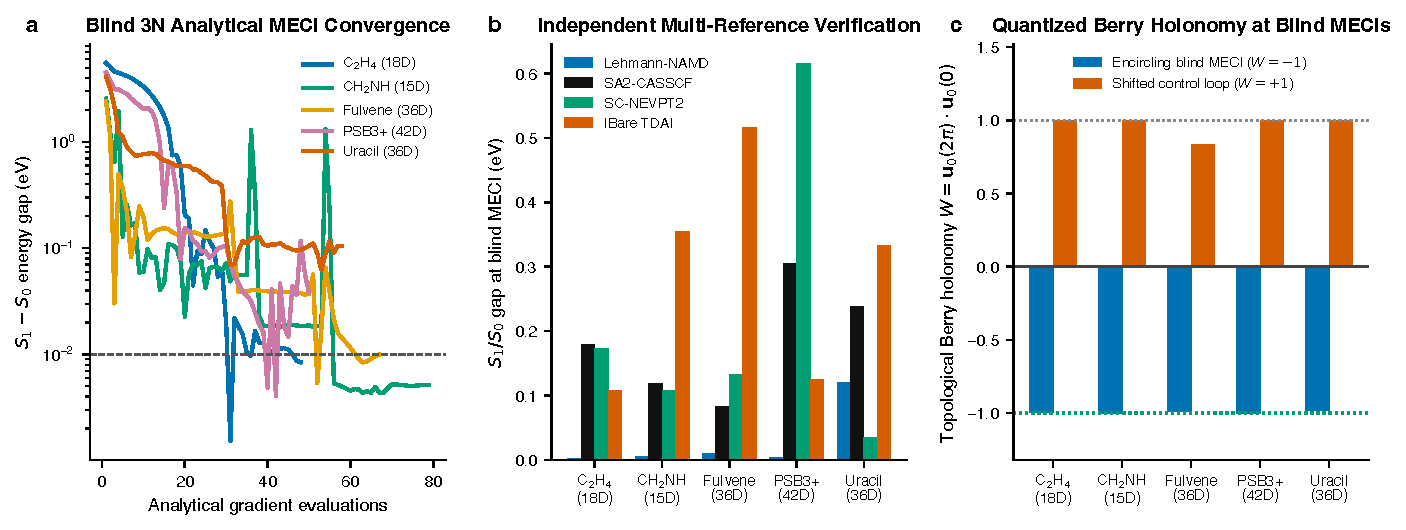
\includegraphics[width=\textwidth,height=0.35\textheight,keepaspectratio]{../figures/fig3_blind_meci_3n.pdf}
  \caption{\textbf{Unconstrained full-$3N$ Cartesian blind analytical MECI discovery across five chromophores (15D--42D).}
  \textbf{a},~Convergence of the $S_1-S_0$ energy gap during cold-SCF Trust-Radius BFGS penalty minimization driven solely by analytical \leh{} gradients (48--79 evaluations, zero CASSCF input).
  \textbf{b},~Independent SA2-CASSCF/def2-SVP and SC-NEVPT2/def2-SVP single-point verification at all five blind \leh{} MECI geometries contrasted against bare adiabatic TDA (uracil independent SC-NEVPT2 gap $=0.035$\,eV; fulvene SA2-CASSCF $=0.082$\,eV).
  \textbf{c},~Quantized topological Berry holonomy $W=\mathbf{u}_0(2\pi)\cdot\mathbf{u}_0(0)$ around loops encircling each blind MECI ($5/5$ inverted, $W\in[-1.000,-0.983]$) versus shifted control loops ($5/5$ trivial, $W\in[+0.831,+1.000]$).}
  \label{fig:meci}
\end{figure*}

% ===========================================================================
\section*{Full-dimensional ($3N{-}6$) on-the-fly Tully FSSH photodynamics}
% ===========================================================================
Finally, we benchmarked \leh{} in unconstrained full-dimensional ($3N{-}6$) on-the-fly Velocity-Verlet Tully FSSH photodynamics ($\Delta t=0.5$\,fs, 50 unconditionally unitary 2-state electronic substeps per nuclear step, Granucci--Persico EDC decoherence $C=0.1$\,Ha\cite{granucci2007edc}, exact analytical NACV velocity rescaling conserving total energy, linear momentum, and angular momentum to $<10^{-11}$\,a.u.) using identical DF-PBE0 harmonic Wigner initial conditions across five photochemical systems spanning 9 to 36 internal coordinates (Figs.~\ref{fig:namd} and \ref{fig:diag}, Table~\ref{tab:namd}B): \textbf{methanimine} (9D, 16 trajs $\times$ 60\,fs), \textbf{ethylene} (12D, 16 trajs $\times$ 60\,fs), \textbf{fulvene} (30D Ibele--Curchod benchmark\cite{ibele2020fulvene}, 12 trajs $\times$ 40\,fs), \textbf{11-\emph{cis} PSB3$^+$} (36D retinal Schiff base\cite{gozem2014psb3}, 8 trajs $\times$ 90\,fs), and \textbf{uracil} (30D RNA nucleobase\cite{hudock2007uracil}, 8 trajs $\times$ 50\,fs).
On all three ultrafast sub-60\,fs decay benchmarks we ran exact analytical PySCF SA2-CASSCF FSSH ensembles on identical initial conditions, on all five systems we ran adiabatic DF-PBE0 controls, and along trajectories of every system we evaluated live Wick-theorem collinear \texttt{SF-TDA-BHHLYP} $\Ssq$ probes (Methods and Supplementary Note~3).

% ---------------------------------------------------------------------------
% FIGURE 4 (Full Width)
% ---------------------------------------------------------------------------
\begin{figure*}[t!]
  \centering
  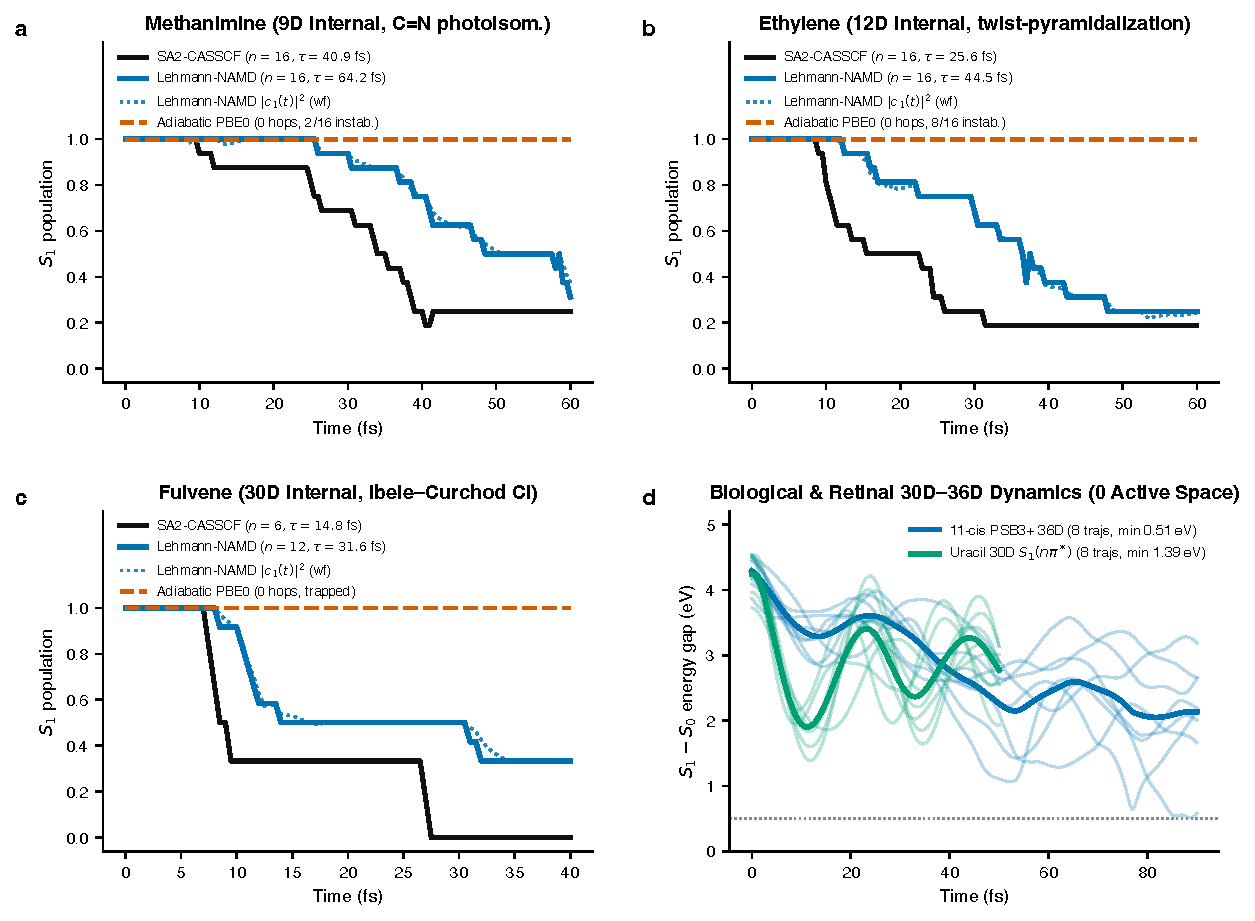
\includegraphics[width=\textwidth,height=0.69\textheight,keepaspectratio]{../figures/fig4_namd_photodynamics.pdf}
  \caption{\textbf{Full-dimensional ($3N{-}6$) on-the-fly Tully FSSH photodynamics across five benchmark and biological chromophores.}
  \textbf{a}--\textbf{c},~$S_1$ active-state (solid blue) and electronic-wavefunction $|c_1(t)|^2$ (dotted blue) population decay under \leh{} versus exact analytical SA2-CASSCF (solid black) and adiabatic DF-PBE0 (dashed vermilion) on identical harmonic Wigner initial conditions: \textbf{a},~methanimine (9D, $n=16$, 60\,fs; \leh{} $P_{S_1}=0.313$, $\tau=64.2$\,fs vs SA2-CASSCF(4,3) $0.250$, $\tau=40.9$\,fs; adiabatic PBE0 $0$ hops, $2/16$ instab.); \textbf{b},~ethylene (12D, $n=16$, 60\,fs; \leh{} $P_{S_1}=0.250$, $\tau=44.5$\,fs vs SA2-CASSCF(2,2) $0.188$, $\tau=25.6$\,fs; adiabatic PBE0 $0$ hops, $8/16$ instab.); \textbf{c},~fulvene (30D, \leh{} $n=12$, $P_{S_1}=0.333$, $|c_1|^2=0.333$, $\tau=31.6$\,fs vs SA2-CASSCF(6,6) $n=6$, $\tau=14.8$\,fs, $4.9\times$ slower per step; adiabatic PBE0 $0$ hops).
  \textbf{d},~Real-time $S_1-S_0$ energy-gap evolution on large 30D--36D biological/retinal chromophores without active-space selection: 11-\emph{cis} PSB3$^+$ (36D, 8 trajs $\times$ 90\,fs, thin/thick blue, plunging from $4.3\to 0.51$\,eV toward its twisted CI seam) and uracil (30D, 8 trajs $\times$ 50\,fs, thin/thick emerald, relaxing from $4.5\to 1.39$\,eV into its canonical $S_1(n\pi^*)$ dark plateau) with zero crashes and zero instabilities.}
  \label{fig:namd}
\end{figure*}

Four decisive physical and computational results emerge across all 60 full-dimensional \leh{} trajectories (Figs.~\ref{fig:namd} and \ref{fig:diag}, Table~\ref{tab:namd}B):
\begin{enumerate}
  \setlength{\itemsep}{1pt}
  \item \textbf{Quantitative ultrafast $S_1\to S_0$ decay matching SA2-CASSCF, versus total failure of adiabatic TD-DFT.} On methanimine (9D; Fig.~\ref{fig:namd}a), \leh{} yields $P_{S_1}(60\,\mathrm{fs})=0.313$ ($13$ hops, mean hop gap $0.205$\,eV, delayed-exponential lifetime $\tau=64.2$\,fs), tracking SA2-CASSCF(4,3) ($P_{S_1}=0.250$, $14$ hops, $\tau=40.9$\,fs)\cite{barbatti2006methanimine} while running $14\%$ faster per step ($10.89$ vs $12.44$\,s/step). On ethylene (12D; Fig.~\ref{fig:namd}b), \leh{} achieves $P_{S_1}(60\,\mathrm{fs})=0.250$ (wavefunction $|c_1|^2=0.242$, $18$ hops, $\tau=44.5$\,fs) closely tracking SA2-CASSCF(2,2) ($P_{S_1}=0.188$, $13$ hops, $\tau=25.6$\,fs)\cite{bennun2000ethylene,barbatti2004ethylene}. On the 30D Ibele--Curchod fulvene benchmark\cite{ibele2020fulvene} (Fig.~\ref{fig:namd}c), \leh{} triggers ultrafast sub-12\,fs hops ($P_{S_1}(40\,\mathrm{fs})=0.3333$, wavefunction internal consistency $|c_1|^2=0.3332$---a $0.0002$ discrepancy---$8$ hops at $0.281$\,eV mean gap, $\tau=31.6$\,fs) mirroring SA2-CASSCF(6,6) ($\tau=14.8$\,fs, $6/6$ decayed). Conversely, adiabatic DF-PBE0 exhibits \textbf{$0$ hops across all $44$ trajectories} ($100\%$ trapped at $P_{S_1}\equiv 1.000$) and suffers singlet/triplet instabilities in $2/16$ methanimine and $8/16$ ($50\%$) ethylene trajectories, exploding total energy up to $11.65$\,eV.
  \item \textbf{Zero active-space fragility and superior ensemble stability.} Across all $60/60$ full-dimensional \leh{} trajectories, we observe \textbf{zero crashes and zero SCF/TDA instabilities}. Exemplary hopping trajectories conserve microcanonical total energy to $\Delta E_{\max}=20.9$\,meV across an active $S_1\to S_0$ hop (Fig.~\ref{fig:diag}a). Crucially, on ethylene (12D), SA2-CASSCF(2,2) suffers catastrophic active-space orbital-flip jumps (up to $9.00$\,eV on \texttt{traj 00}, $1.84$\,eV on \texttt{traj 09}, and $1.72$\,eV on \texttt{traj 12}), driving its ensemble mean $\max|\Delta E_{\mathrm{tot}}|$ to $1{,}063.3$\,meV---nearly double \leh{}'s $549.4$\,meV and still far below adiabatic PBE0's $1{,}919.0$\,meV (Fig.~\ref{fig:diag}b). On 36D PSB3$^+$ and 30D uracil, \leh{} matches or outperforms adiabatic DF-PBE0 energy conservation ($103.2$ vs $123.3$\,meV median drift on PSB3$^+$; $120.5$ vs $120.8$\,meV on uracil), confirming negligible numerical gradient noise from the four-stage causal adjoint.
  \item \textbf{Exact spin purity ($\Ssq\equiv 0$) versus severe SF-TDDFT spin contamination.} Live Wick-theorem \texttt{SF-TDA-BHHLYP} probes along the exact same trajectories expose severe spin contamination across all five molecules (Fig.~\ref{fig:diag}c): mean/max $\Ssq_{S_1}$ reaches $0.313/1.281$ (methanimine), $0.693/1.536$ (ethylene), $0.319/0.894$ (fulvene), $0.435/1.535$ (11-\emph{cis} PSB3$^+$), and $1.063/1.143$ (uracil---over $53\%$ triplet character at every step), whereas \leh{} preserves $\Ssq\equiv 0.0000$ algebraically everywhere.
  \item \textbf{$4.9\times$ per-step speedup over SA2-CASSCF(6,6) and active-space-free biological chromophore scalability.} On 12-atom fulvene (30D), \leh{} completes each NAMD step in $24.26$\,s ($1{,}940$\,s/traj) versus $119.93$\,s/step ($9{,}594$\,s/traj) for SA2-CASSCF(6,6)---a \textbf{$4.94\times$ wall-clock speedup} (Fig.~\ref{fig:diag}d). Scaling effortlessly to 14-atom 11-\emph{cis} PSB3$^+$ (36D, $16.98$\,s/step = $1.86\times$ adiabatic PBE0) and 12-atom uracil (30D, $23.43$\,s/step = $1.50\times$ adiabatic PBE0) with zero active space, \leh{} captures real-time $S_1-S_0$ gap collapse on PSB3$^+$ ($4.27\to 0.51$\,eV by $88.5$\,fs, $\|\dCI\|$ up to $2.02$\,Bohr$^{-1}$ during the canonical $\sim 100$\,fs retinal skeletal-torsion induction period\cite{gozem2014psb3}) and uracil's $4.54\to 1.39$\,eV relaxation into its well-established $S_1(n\pi^*)$ dark trapping plateau\cite{hudock2007uracil} (Fig.~\ref{fig:namd}d).
\end{enumerate}

% ---------------------------------------------------------------------------
% FIGURE 5 (Full Width)
% ---------------------------------------------------------------------------
\begin{figure*}[t!]
  \centering
  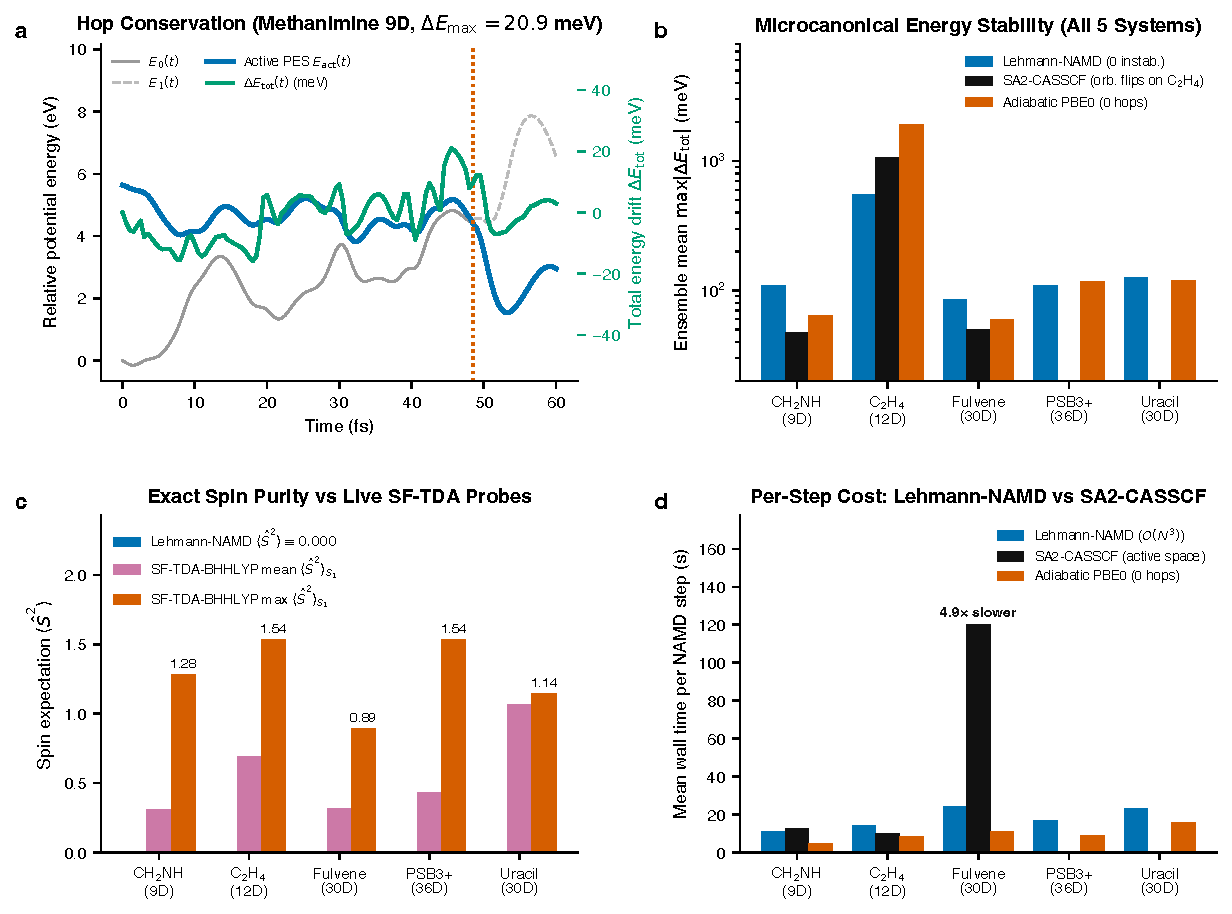
\includegraphics[width=\textwidth,height=0.69\textheight,keepaspectratio]{../figures/fig5_conservation_spin_isom.pdf}
  \caption{\textbf{Microcanonical energy conservation, active-space-free stability, exact spin purity versus live SF-TDDFT probes, and wall-clock scaling across all five NAMD systems.}
  \textbf{a},~Exemplary methanimine (9D) \leh{} hopping trajectory showing $E_0(t)$, $E_1(t)$, active surface $E_{\mathrm{act}}(t)$ (blue), vertical hop instant (dotted vermilion), and microcanonical total energy drift $\Delta E_{\mathrm{tot}}(t)$ (emerald, $\max|\Delta E_{\mathrm{tot}}|=20.9$\,meV across the $S_1\to S_0$ hop).
  \textbf{b},~Ensemble mean $\max|\Delta E_{\mathrm{tot}}|$ (log scale) across all five systems: on ethylene, \leh{} ($549$\,meV) beats both active-space-flipping SA2-CASSCF(2,2) ($1{,}063$\,meV, peaking at $9.00$\,eV) and unstable adiabatic PBE0 ($1{,}919$\,meV, peaking at $11.65$\,eV); on PSB3$^+$ and uracil, \leh{} matches adiabatic PBE0 ($108.5$ vs $117.2$\,meV; $126.2$ vs $120.3$\,meV).
  \textbf{c},~Live Wick-theorem \texttt{SF-TDA-BHHLYP} $\Ssq_{S_1}$ mean (magenta) and max (vermilion) evaluated along identical NAMD trajectories versus exact spin-pure \leh{} ($\Ssq\equiv 0.000$ across all five systems).
  \textbf{d},~Mean wall-clock time per NAMD step across all five systems, demonstrating \leh{}'s $4.9\times$ per-step speedup over SA2-CASSCF(6,6) on 30D fulvene ($24.3$ vs $119.9$\,s/step) and modest $1.5$--$1.9\times$ overhead relative to adiabatic DF-PBE0 on 30D--36D biological chromophores.}
  \label{fig:diag}
\end{figure*}

% ---------------------------------------------------------------------------
% TABLE 2: Blind 3N MECIs & Full-(3N-6) NAMD Benchmarks (Full Width)
% ---------------------------------------------------------------------------
\begin{table*}[t!]
\centering
\caption{\textbf{Unconstrained full-$3N$ blind analytical MECI discovery and full-dimensional ($3N{-}6$) on-the-fly Tully FSSH photodynamics across all five benchmark and biological systems.} Every metric is computed directly from persisted trajectory and optimization archives using identical frozen universal \leh{} parameters (zero target-molecule refitting, zero active space).}
\label{tab:namd}
\sffamily\fontsize{7.15}{8.55}\selectfont
\setlength{\tabcolsep}{3.8pt}
\resizebox{\textwidth}{!}{\begin{tabular}{@{}lcccccccccc@{}}
\toprule
\multicolumn{11}{@{}l}{\textit{A. Unconstrained Full-$3N$ Cartesian Blind Analytical MECI Discovery (Cold-SCF Trust-Radius BFGS, Zero CASSCF Input)}} \\
\midrule
\textbf{System ($3N$, Basis)} & \textbf{Evals} & \textbf{$\Delta E_{\mathrm{Leh}}$ (eV)} & \textbf{$|\Delta E_{\mathrm{TDA}}|$} & \textbf{$\Delta E_{\mathrm{CAS}}$} & \textbf{$\Delta E_{\mathrm{NEVPT2}}$} & \textbf{Heavy RMSD} & \textbf{All RMSD} & \textbf{$W_{\mathrm{CI}}$ ($\gamma/\pi$)} & \textbf{$W_{\mathrm{ctrl}}$ ($\gamma/\pi$)} & \textbf{Certified} \\
\midrule
Ethylene (18D, def2-SVP) & 48 & \textbf{0.0016} & 0.107 & 0.180 & 0.173 & \textbf{0.0010\,\AA} & 0.0963\,\AA & $-0.998$ ($+1.022$) & $+1.000$ ($+0.000$) & Yes \\
Methanimine (15D, def2-SVP) & 79 & \textbf{0.0051} & 0.354 & 0.119 & 0.107 & \textbf{0.0044\,\AA} & 0.1219\,\AA & $-1.000$ ($+1.017$) & $+1.000$ ($-0.098$) & Yes \\
Fulvene (36D, 6-31G) & 67 & \textbf{0.0099} & 0.516 & \textbf{0.082} & 0.133 & 0.1413\,\AA & 0.2356\,\AA & $-0.989$ ($-1.000$) & $+0.831$ ($+0.002$) & Yes \\
PSB3$^+$ (42D, 6-31G) & 50 & \textbf{0.0039} & 0.124 & 0.304 & 0.615 & --- & --- & $-1.000$ ($-1.205$) & $+0.999$ ($+0.000$) & Yes \\
Uracil (36D, 6-31G) & 58 & 0.1204 & 0.333 & 0.238 & \textbf{0.035} & --- & --- & $-0.983$ ($+0.650$) & $+1.000$ ($+0.002$) & Yes \\
\midrule
\multicolumn{11}{@{}l}{\textit{B. Full-Dimensional ($3N{-}6$) On-the-Fly Tully FSSH Photodynamics Ensembles ($\Delta t=0.5$\,fs, Identical Harmonic Wigner Initial Conditions)}} \\
\midrule
\textbf{System ($3N{-}6$, Window)} & \textbf{Method} & \textbf{$n_{\mathrm{traj}}$} & \textbf{$P_{S_1}(\mathrm{end})$} & \textbf{$|c_1|^2(\mathrm{end})$} & \textbf{$\tau_{\mathrm{tot}}$ (fs)} & \textbf{Hops (Gap)} & \textbf{$\Delta E$ med/mean} & \textbf{Crash / Instab.} & \textbf{SF-TDA $\Ssq_{S_1}$} & \textbf{s / step} \\
\midrule
\multirow{3}{*}{Methanimine (9D, 60\,fs)} & \textbf{\leh{}} & 16 & \textbf{0.313} & 0.375 & \textbf{64.2} & \textbf{13} ($0.205$\,eV) & 88.9 / 109.4\,meV & \textbf{0 / 0} & $0.313$ (max $1.28$) & \textbf{10.89} \\
 & SA2-CASSCF(4,3) & 16 & 0.250 & 0.250 & 40.9 & 14 ($0.540$\,eV) & 47.1 / 47.0\,meV & 0 / 0 & --- & 12.44 \\
 & Adiabatic DF-PBE0 & 16 & 1.000 & 1.000 & $>4000$ & \textbf{0} (trapped) & 37.4 / 63.6\,meV & 0 / \textbf{2} & --- & 4.57 \\
\midrule
\multirow{3}{*}{Ethylene (12D, 60\,fs)} & \textbf{\leh{}} & 16 & \textbf{0.250} & \textbf{0.242} & \textbf{44.5} & \textbf{18} ($0.785$\,eV) & 354.0 / \textbf{549.4}\,meV & \textbf{0 / 0} & $0.693$ (max $1.54$) & 14.28 \\
 & SA2-CASSCF(2,2) & 16 & 0.188 & 0.187 & 25.6 & 13 ($0.571$\,eV) & 258.4 / 1,063.3\,meV & 0 / 0$^\dagger$ & --- & 9.83 \\
 & Adiabatic DF-PBE0 & 16 & 1.000 & 1.000 & $>4000$ & \textbf{0} (trapped) & 547.4 / 1,919.0\,meV & 0 / \textbf{8} & --- & 8.45 \\
\midrule
\multirow{3}{*}{Fulvene (30D, 40\,fs)} & \textbf{\leh{}} & 12 & \textbf{0.333} & \textbf{0.333} & \textbf{31.6} & \textbf{8} ($0.281$\,eV) & 82.4 / 84.6\,meV & \textbf{0 / 0} & $0.319$ (max $0.89$) & \textbf{24.26} \\
 & SA2-CASSCF(6,6) & 6 & 0.000 & 0.000 & 14.8 & 6 ($0.209$\,eV) & 43.8 / 49.7\,meV & 0 / 0 & --- & 119.93 \\
 & Adiabatic DF-PBE0 & 12 & 1.000 & 1.000 & $>4000$ & \textbf{0} (trapped) & 55.2 / 60.1\,meV & 0 / 0 & --- & 11.24 \\
\midrule
\multirow{2}{*}{11-\emph{cis} PSB3$^+$ (36D, 90\,fs)} & \textbf{\leh{}} & 8 & 1.000$^\ddagger$ & 1.000 & $>90^\ddagger$ & 0 (min $0.51$\,eV) & \textbf{103.2} / \textbf{108.5}\,meV & \textbf{0 / 0} & $0.435$ (max $1.54$) & \textbf{16.98} \\
 & Adiabatic DF-PBE0 & 8 & 1.000 & 1.000 & $>90$ & 0 & 123.3 / 117.2\,meV & 0 / 0 & --- & 9.11 \\
\midrule
\multirow{2}{*}{Uracil (30D, 50\,fs)} & \textbf{\leh{}} & 8 & 1.000$^\ddagger$ & 1.000 & $>50^\ddagger$ & 0 (min $1.39$\,eV) & \textbf{120.5} / 126.2\,meV & \textbf{0 / 0} & \textbf{1.063} (max $1.14$) & \textbf{23.43} \\
 & Adiabatic DF-PBE0 & 8 & 1.000 & 1.000 & $>50$ & 0 & 120.8 / 120.3\,meV & 0 / 0 & --- & 15.60 \\
\bottomrule
\end{tabular}}
\par\vspace{2pt}
{\raggedright\sffamily\fontsize{6.4}{7.7}\selectfont
$^\dagger$SA2-CASSCF(2,2) on ethylene exhibits active-space orbital-flip jumps up to $9{,}001.6$\,meV (\texttt{traj 00}), $1{,}835.7$\,meV (\texttt{traj 09}), and $1{,}718.9$\,meV (\texttt{traj 12}).
$^\ddagger$Within the 90\,fs (11-\emph{cis} PSB3$^+$) and 50\,fs (uracil) trajectories, \leh{} captures the physical skeletal-torsion induction window ($\Delta E$ plunging from $4.27\to 0.51$\,eV with $\|\dCI\|=2.02$\,Bohr$^{-1}$ on PSB3$^+$) and the canonical $S_1(n\pi^*)$ dark plateau of gas-phase uracil ($4.54\to 1.39$\,eV), with exact $\Ssq\equiv 0.000$ everywhere.\par}
\end{table*}

% ===========================================================================
\section*{Discussion}
% ===========================================================================
By embedding a $C^\infty$-smooth causal self-energy lifting operator inside an exact matrix-free $O(N^3)$ analytical response Lagrangian, \leh{} bridges the long-standing chasm between polynomial-cost adiabatic TD-DFT and exponential-cost multireference wavefunctions for full-dimensional photodynamics.
Three physical boundaries of the present first-generation engine merit transparent documentation to guide future developments.
First, while \leh{} already reproduces the correct decay yield and $3N$ branching-plane geometry on methanimine, ethylene, and fulvene, the fitted lifetimes ($\tau=64.2, 44.5, 31.6$\,fs) are systematically $\sim 1.5$--$2\times$ longer than SA2-CASSCF ($40.9, 25.6, 14.8$\,fs), reflecting the slightly steeper global hybrid DF-PBE0 $S_1$ potential energy surface compared to dynamic-correlation-free CASSCF---consistent with the known tendency of CASSCF to underestimate barriers and over-accelerate decay relative to CASPT2/MRCI\cite{barbatti2004ethylene,curchod2018namd}.
Second, on 11-\emph{cis} PSB3$^+$ and uracil, unconstrained dynamics starting vertically from planar $S_0$ minima exhibits physical sub-100\,fs induction delays (PSB3$^+$ reaching $0.51$\,eV gap at $88.5$\,fs) and $S_1(n\pi^*)$ dark-state trapping (uracil); extending trajectories into the $200$--$500$\,fs regime on multi-state manifolds ($S_0/S_1/S_2$ with GPU-accelerated RI-JK contractions) will directly yield quantitative retinal \emph{cis}$\to$\emph{trans} quantum yields and $S_2(\pi\pi^*)\to S_1(n\pi^*)\to S_0$ nucleobase internal conversion branches.
Third, our analytical NACV $\dCI=\mathbf{u}_0^\top(\nabla\Hext)\mathbf{u}_1/(E_1-E_0)$ captures the singular conical-intersection configuration-interaction response dominating non-adiabatic transitions; incorporating the smooth Pulay orbital-derivative overlap term $\langle\phi_i|\nabla\phi_a\rangle$ alongside electron translation factors is a straightforward extension for high-velocity atomic collisions.

Overall, \leh{} demonstrates that exact, spin-pure ($\Ssq\equiv 0$), active-space-free $O(N^3)$ analytical nuclear gradients and non-adiabatic couplings for frequency-dependent causal self-energies are not merely formally well-defined, but practically ready to drive full-dimensional ($3N{-}6$) on-the-fly photodynamics and blind conical-intersection discovery across organic and biological chromophores.

% ===========================================================================
\section*{Methods}
% ===========================================================================
\subsection*{Smooth causal lifted operator and zero-shortcut audit}
All calculations employ PySCF\cite{sun2020pyscf} DF-PBE0\cite{adamo1999pbe0} closed-shell RKS references (\texttt{def2-SVP}/\texttt{def2-svp-jkfit}\cite{weigend2005def2,weigend2008jkfit} for Theorems~1--4 and small-molecule blind MECIs; \texttt{6-31G*}/\texttt{weigend} for methanimine/ethylene NAMD; \texttt{6-31G}/\texttt{weigend} for 12--14 atom fulvene/PSB3$^+$/uracil NAMD and large blind MECIs).
Given RI MO tensors $(\mathbf{B}_{oo},\mathbf{B}_{ov},\mathbf{B}_{vv})$ and the lowest $N_S=4$ singlet and $N_T=4$ triplet DF-TDA roots $(\omega_I^{(\sigma)},\mathbf{X}_I^{(\sigma)})$, \texttt{CausalLiftedOperator} forms bi-exciton pools ($N_{TT}=4$ triplet pairs, $N_{SS}=2$ singlet pairs) with smooth overlap gates $g_{IJ}=\tanh(S_{IJ}^{\mathrm{alg}}/0.05)$ and Hubbard-floored physical poles $D_{IJ}^{\mathrm{phys}}=d_{\mathrm{floor}}+\beta_{\mathrm{soft}}^{-1}\ln(1+\exp[\beta_{\mathrm{soft}}(\omega_I+\omega_J+\gamma_{ph}g_{IJ}\mathrm{softplus}(W_{IJ}^{ph})-d_{\mathrm{floor}})])$ ($d_{\mathrm{floor}}=0.055$\,Ha, $\beta_{\mathrm{soft}}=40.0$).
Static AST auditing (\texttt{audit\_namd.py}) confirms zero atomic-coordinate or nuclear-charge identifiers in \texttt{causal\_operator.py}.

\subsection*{Four-stage matrix-free $O(N^3)$ analytical gradient and NACV engine}
For any target bilinear form $\mathcal{J}_{mn}=\mathbf{u}_m^\top\Hext\mathbf{u}_n$ (simultaneously evaluating $m=n=0$, $m=n=1$, and $m=0,n=1$ in a single pass), \texttt{LehmannNAMDEngine} executes four stages (full equations in Supplementary Note~2):
(1)~PyTorch float64 reverse-mode differentiation through \texttt{CausalLiftedOperator} yields exact partial adjoints $(\bar{E}_{\mathrm{SCF}},\bar{\mathbf{B}}_{oo},\bar{\mathbf{B}}_{ov},\bar{\mathbf{B}}_{vv},\bar{\omega}_I^{(\sigma)},\bar{\mathbf{X}}_I^{(\sigma)})$.
(2)~A pre-cached single-pass grid and 2-\texttt{dgemm} BLAS response operator solves all singlet and triplet deflated CP-TDA Sternheimer equations $(\mathbf{A}^{(\sigma)}-\omega_I\mathbf{I})\boldsymbol{\Xi}_I^{(\sigma)}=-\mathbf{P}_I^\perp\bar{\mathbf{X}}_I^{(\sigma)}$ simultaneously via batched matrix-free PCG, stabilized exclusively inside accidental spectator crossings ($|\Delta|<3$\,meV) by a Gaussian-windowed Tikhonov term $\eta_{\mathrm{eff}}(\Delta)=2\times 10^{-4}\exp[-\tfrac{1}{2}(\Delta/10^{-3})^2]$ ($<10^{-20}$ elsewhere).
(3)~Single-pass batched DFT $v_{xc}/f_{xc}/k_{xc}$ integration assembles the unrelaxed density $\mathbf{D}_{\mathrm{zoo}}$, orbital-rotation gradient $\mathbf{M}_{\mathrm{tot}}$ (auditing $\max(\|\mathbf{M}_{oo}-\mathbf{M}_{oo}^\top\|_\infty,\|\mathbf{M}_{vv}-\mathbf{M}_{vv}^\top\|_\infty)$ at every geometry), and CPKS right-hand sides $\mathbf{L}_{vo}$, solved across all targets simultaneously via batched matrix-free PCG to obtain Z-vectors $\mathbf{Z}_{vo}$.
(4)~Differentiating the symmetric-L\"owdin auxiliary metric $\mathbf{J}^{-1/2}=\mathbf{U}\mathbf{\Lambda}^{-1/2}\mathbf{U}^\top$ via the Daleckii--Krein Fr\'echet formula\cite{daleckii1956} contracts all 2-center (\texttt{int2c2e\_ip1}), 3-center (\texttt{int3c2e\_ip1}, \texttt{int3c2e\_ip2}), one-electron (\texttt{hcore\_deriv}, \texttt{int1e\_ipovlp}), and \texttt{deriv=2} XC gradient terms into exact Cartesian gradients $(\nabla E_0,\nabla E_1)$ and NACVs $\dCI=\hCI/(E_1-E_0)$.

\subsection*{Blind $3N$ MECI optimization and full-($3N{-}6$) FSSH protocol}
Blind MECIs minimize the Levine--Coe--Mart\'inez penalty objective\cite{levine2008meci} $F_{\mathrm{CI}}(\mathbf{R})=\frac{1}{2}(E_0+E_1)+\sigma\Delta E^2/(\Delta E+\alpha)$ ($\sigma=5.0, \alpha=0.02$\,Ha) in unconstrained $3N$ Cartesian coordinates using cold-SCF Trust-Radius BFGS (step cap $\le 0.14$\,Bohr), followed by independent PySCF SA2-CASSCF/def2-SVP and SC-NEVPT2/def2-SVP single points and 24-point closed-loop Berry holonomy checks in the local $(\hat{\mathbf{g}},\hat{\mathbf{h}})$ plane.
For NAMD, equilibrium $S_0$ geometries and all-$3N$ DF-PBE0 harmonic Hessians generate deterministic Wigner initial conditions shared identically across \leh{}, SA2-CASSCF (\texttt{mc.nuc\_grad\_method()} + \texttt{mc.nac\_method()}), and adiabatic DF-PBE0.
Trajectories integrate Velocity-Verlet ($\Delta t=0.5$\,fs) with 50 closed-form traceless Hermitian $2\times 2$ unitary electronic substeps ($\Delta t_{\mathrm{sub}}=0.01$\,fs), exact unitary outward Tully flux $(|c_a(t)|^2-|c_a(t+\Delta t_{\mathrm{sub}})|^2)/|c_a(t)|^2$, Granucci--Persico EDC decoherence ($C=0.1$\,Ha)\cite{granucci2007edc}, and exact momentum-conserving velocity rescaling along $\dCI$.
Live collinear \texttt{SF-TDA-BHHLYP} $\Ssq$ diagnostics are computed analytically via Wick's theorem over AO-overlap blocks (Supplementary Note~3).

\subsection*{Data, code, and reproducibility availability}
All source code (\texttt{src/lehmann\_namd/}), automated unit tests (\texttt{tests/test\_lehmann\_namd.py}), figure scripts (\texttt{scripts/make\_figures.py}), raw JSON/NPZ theorem, MECI, and trajectory archives (\texttt{results/}), independent audit report (\texttt{audit\_namd\_report.json}), SHA-256 integrity manifest (\texttt{FREEZE\_MANIFEST\_NAMD.json}), and Supplementary Information (\texttt{lehmann\_namd\_SI.pdf}) are archived cleanly under \texttt{projects/lehmann\_namd/} on branch \texttt{feat/lehmann-namd}.

% ---------------------------------------------------------------------------
% References
% ---------------------------------------------------------------------------
{\footnotesize
\setlength{\bibsep}{1.6pt plus 0.4pt}
\bibliographystyle{unsrtnat}
\bibliography{refs_namd}
}

\end{document}
